\section{Soll-Ist-Zeit-Vergleich}
Während des ganzen Projektes haben wir in Jira vor jeder Phase die jeweiligen Tasks definiert und den Aufwand dazu geschätzt (Soll). Weiter haben wir dann auch die effektive Zeit zu den Tasks erfasst (Ist).
\subsection{Inception}
\begin{tabbing}[H]
    \hspace*{3cm}\=\hspace*{5cm}\=\hspace*{3cm}\=\hspace*{3cm}\= \kill
    Start: \> 14.09.2015 \>	Ende: \> 23.09.2015 \\
\end{tabbing}
\begin{figure}[H]
\centering
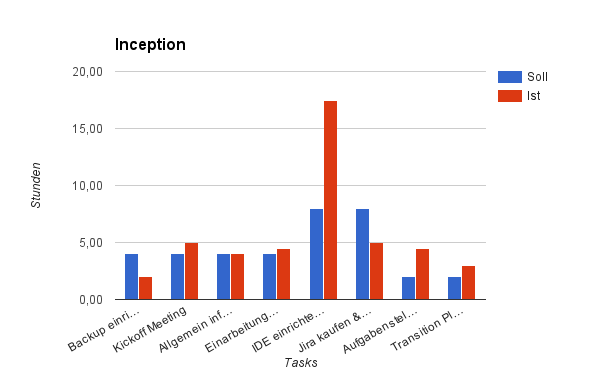
\includegraphics[width=390pt]{images/inception.png}
\caption[Inception]{Inception}
\end{figure}
\newpage
\subsection{Elaboration1}
\begin{tabbing}[H]
    \hspace*{3cm}\=\hspace*{5cm}\=\hspace*{3cm}\=\hspace*{3cm}\= \kill
    Start: \> 23.09.2015 \> Ende: \> 19.10.2015 \\
\end{tabbing}
\begin{figure}[H]
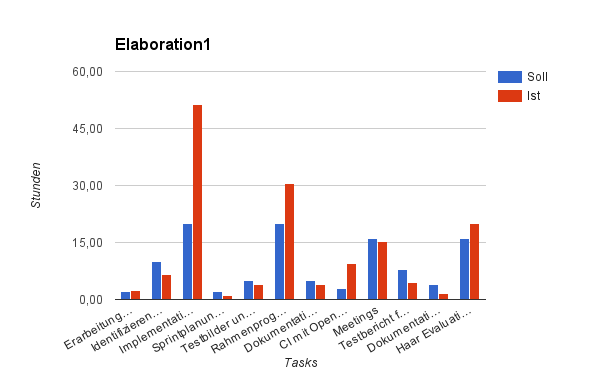
\includegraphics[width=390pt]{images/elab1.png}
\caption[Elaboration1]{Elaboration1}
\end{figure}

\subsection{Elaboration2}
\begin{tabbing}[H]
    \hspace*{3cm}\=\hspace*{5cm}\=\hspace*{3cm}\=\hspace*{3cm}\= \kill
    Start: \> 19.10.2015 \> Ende: \>  04.11.2015 \\
\end{tabbing}
\begin{figure}[H]
\centering
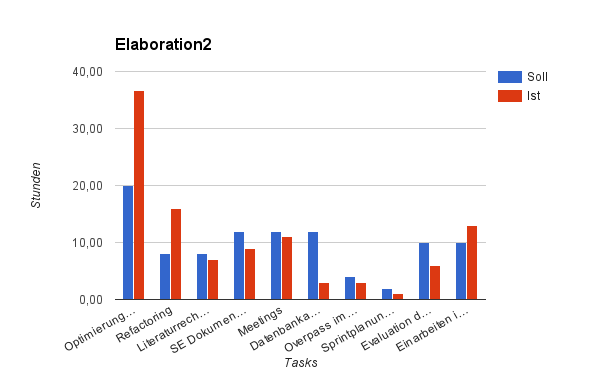
\includegraphics[width=390pt]{images/elab2.png}
\caption[Elaboration2]{Elaboration2}
\end{figure}

\subsection{Construction1}
\begin{tabbing}[H]
    \hspace*{3cm}\=\hspace*{5cm}\=\hspace*{3cm}\=\hspace*{3cm}\= \kill
    Start: \> 04.11.2015 \>	Ende: \>  25.11.2015 \\
\end{tabbing}
\begin{figure}[H]
\centering
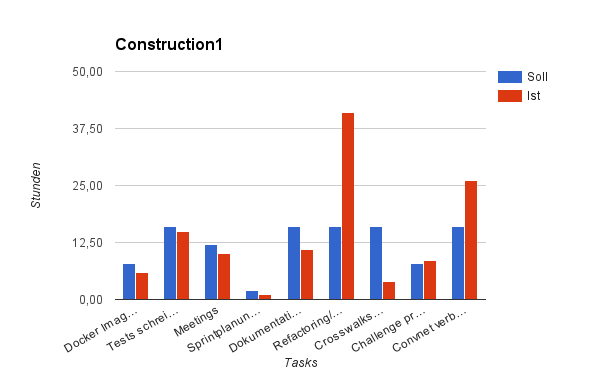
\includegraphics[width=390pt]{images/construction1.png}
\caption[Construction1]{Construction1}
\end{figure}

\subsection{Construction2}
\begin{tabbing}[H]
    \hspace*{3cm}\=\hspace*{5cm}\=\hspace*{3cm}\=\hspace*{3cm}\= \kill
    Start: \> 04.11.2015 \>	Ende: \>  11.11.2015 \\
\end{tabbing}
\begin{figure}[H]
\centering
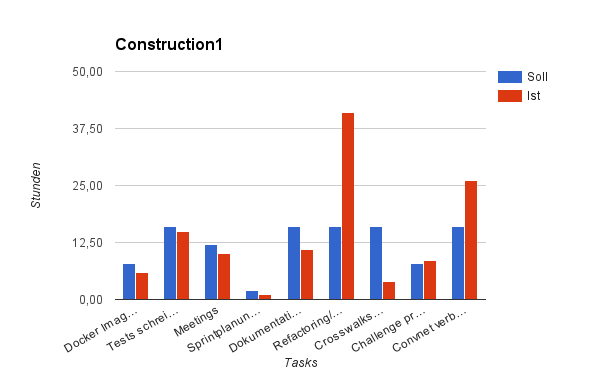
\includegraphics[width=390pt]{images/construction1.png}
\caption[Construction2]{Construction2}
\end{figure}

\subsection{Transition}
\begin{tabbing}[H]
    \hspace*{3cm}\=\hspace*{5cm}\=\hspace*{3cm}\=\hspace*{3cm}\= \kill
    Start: \> 11.12.2015 \> Ende: \>  18.12.2015 \\
\end{tabbing}
\begin{figure}[H]
\centering
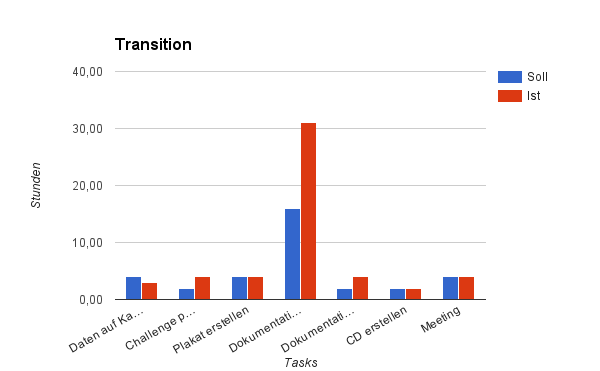
\includegraphics[width=390pt]{images/transition.png}
\caption[Transition]{Transition}
\end{figure}

\subsection{Übersicht}
\begin{table}[H]
\centering
    \begin{tabular}{|p{5cm}|p{2cm}|p{2cm}|p{2cm}|}
    \hline    
    \rowcolor{lightblue}
	Phase & Soll & Ist & Differenz \\ \hline
	Inception & 36.00 &	45.50 &	9.50 \\ \hline
	Elaboration1 & 111.00 & 150.50	& 39.50 \\ \hline
	Elaboration2 & 98.00 & 105.75 & 7.75 \\ \hline
	Construction1 & 110.00 & 122.50 & 12.50 \\ \hline
	Construction1 & 58.00 & 88.50 & 30.50 \\ \hline
	Transition & 34.00 & 52.00 & 18.00 \\ \hline
	\rowcolor{lightblue}
	Total & 447.00 & 564.75 & 117.75 \\ \hline
    \end{tabular}
    \caption[Phasen]{Phasen}
\end{table}
\medskip
Schätzen ist wie bekannt, ein relativ schwierige Angelegenheit. So haben wir den Aufwand für die jeweiligen Tasks meist zu tief eingestuft. Stark ins Gewicht fiel die Evaluation und Implementierung des Bilderkennungsalgorithmus.

\newpage